\documentclass[a4paper,12pt,fleqn]{article}
\usepackage[T1]{fontenc}
\usepackage[utf8]{inputenc}
\usepackage[polish]{babel}
\usepackage{amssymb}
\usepackage{amsthm}
\usepackage{times}
\usepackage{anysize}
\usepackage{graphicx}

\marginsize{1.5cm}{1.5cm}{1.5cm}{1.5cm}
\sloppy 

\theoremstyle{definition}
\newtheorem{df}{Definicja}


\begin{document}

%\maketitle

\section*{Całka Riemanna}

Niech dana będzie funkcja ograniczona $f \colon [a,b] \rightarrow \mathbb{R}$. Sumą częściową (Riemanna) nazywa się liczbę

\begin{equation}
R_{f,P(q_{1}, \dots , q_{2})} = \sum_{i=1}^{n} f(q_{i})\cdot \Delta p_{i}
\end{equation}

\noindent
Funkcję $f$ nazywa się \emph{całkowalną w sensie Riemanna} lub krótko \emph{R-całkowalną}, jeśli dla dowolnego ciągu normalnego $(P^{k})$ podziałów przedziału $[a,b]$, istnieje (niezależna od wyboru punktów pośrednich) granica

$$
R_{f} = \lim_{k \rightarrow \inf} R_{f, P^{k}(q_{1}^{k}, \dots q_{n_{k}}^{k})}
$$

\noindent
nazywana wtedy \textbf{całką Riemanna} tej funkcji. Równoważnie: jeżeli istnieje taka liczba $R_{f}$, że dla dowolnej liczby rzeczywistej $\varepsilon > 0$ istnieje taka liczba rzeczywista $\delta > 0$, że dla dowolnego podziału $P(q_{1}, \dots , q_{n})$ o średnicy $diam P(q_{1}, \dots , q_{n}) < \delta;$ bądź też w języku rozdrobnień: że dla dowolnej liczby rzeczywistej $\varepsilon > 0$ istnieje taki podział $S(t_{1}, \dots , t_{m})$ przedziału $\left[ a,b \right]$, że dla każdego podziału $P(q_{1}, \dots , q_{n})$ rozdrabniającego $S(t_{1}, \dots , t_{m})$ zachodzi

$$
\left| R_{f, P(q_{1}, \dots q_{n})} - R_{f} \right| < \varepsilon
$$

\begin{figure}[!htb]
\centerline{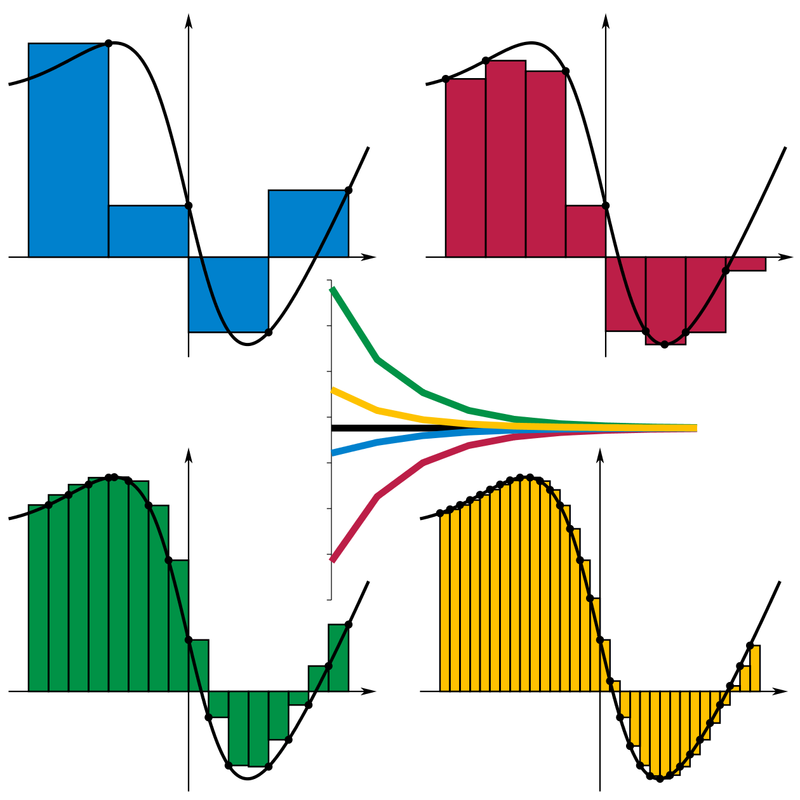
\includegraphics[scale=1.5]{wykresy.png}}
\label{fig:ukladPrzekaznikowy}
\end{figure}

\end{document}

